\footnotesize
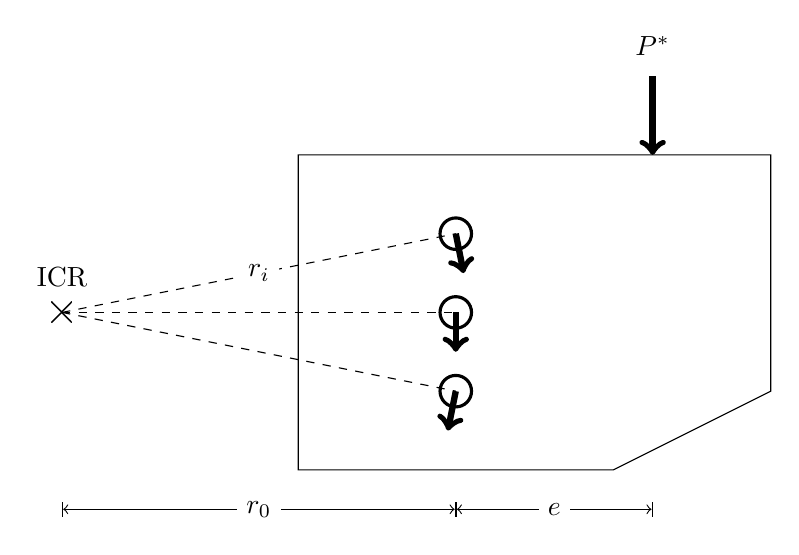
\begin{tikzpicture}
\draw(-1,-1)--++(4,0)--++(2,1)--++(0,3)-|cycle;
\foreach\x in{1}{
\foreach\y in{0,1,2}{
\draw(\x,\y)node[circle,inner sep=0pt,minimum size=4mm,line width=.4mm,draw]{};}}
\draw[->,line width=.8mm](3.5,4)node[above=1mm]{$P^*$}--++(0,-1);
\draw[|<->|](1,-1.5)--(3.5,-1.5)node[midway,fill=white]{$e$};
\draw[|<->|](-4,-1.5)--(1,-1.5)node[midway,fill=white]{$r_0$};
\draw[dashed](-4,1)node{\LARGE\texttimes}node[above=2mm]{ICR}--(1,1);
\draw[dashed](-4,1)--(1,2)node[midway,fill=white]{$r_i$}(-4,1)--(1,0);
\draw[->,line width=.8mm](1,2)--++(.1,-.5);
\draw[->,line width=.8mm](1,1)--++(0,-.5);
\draw[->,line width=.8mm](1,0)--++(-.1,-.5);
\end{tikzpicture}